\section{Versuchsaufbau}
\label{sec:durchfuehrung}
Das Kugelfall-Viskosimeter nach Höppler besteht aus einem zylinderförmigen Glasrohr,
das mit einer Flüssigkeit gefüllt wird (hier destilliertes Wasser), deren Viskosität bestimmt werden soll. 
In dem befüllten Rohr wird eine Kugel fallen gelassen, deren Durchmesser nahe am Rohrdurchmeser liegt.
Es werden hier zwei Kugeln mit unterschiedlichen Durchmessern verwendet. 
Um unkontrollierte Stöße mit der Rohrwand und Wirbelbildungen zu vermeiden, wird das Rohr etwas geneigt.
Am Rohr befinden sich insgesamt drei Markierungen, die je einen Abstand von 5 Zentimetern zueinander haben.
Am Viskosimeter befindet sich eine Libelle, mit der überprüft werden kann, ob das Viskosimeter gerade steht.
Das Viskosimeter selbst ist in Abbildung \ref{fig:viskosimeter} zu sehen.
\begin{figure}
    \centering
    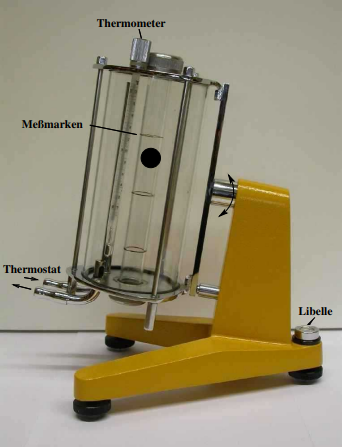
\includegraphics[]{versuchsaufbau.png}
    \caption[]{Foto des Viskosimeters}
    \label{fig:viskosimeter}
\end{figure}
Das Fallrohr befindet sich in einem Wasserbad, durch das mit Hilfe eines angeschlossenen Thermostates die Temperatur im Rohr geregelt werden kann.
Am Thermostat befindet sich ein Thermometer, sodass die Temperatur im Viskosimeter abgelesen werden kann.

\section{Durchführung}
Bei der Durchführung ist mit Hilfe der Libelle darauf zu achten, dass der Fuß des Viskosimeters zu jedem Zeitpunkt gerade steht
bzw. gleichermaßen geneigt ist.
Generell sei angemerkt, dass das Viskosimeter um 180° gedreht werden kann. 
Da durch die Neigung des Fallrohrs allerdings kleine Winkelunterschiede nach der Drehung vorhanden sind, werden bei jeder Messreihe Werte aufgenommen,
bei denen die Kugel von dem oberen zum unteren Ende des Rohres fällt, und Werte, bei denen sie nach der Drehung in die umgekehrte Richtung fällt.
Dementsprechend werden im Folgenden die Werte mit \enquote{oben} betitelt, falls die Kugel von oben fällt, und \enquote{unten}, falls sie von unten fällt.
Zu Beginn des Versuchs werden die Durchmesser der beiden Kugeln mit Hilfe einer Schieblehre bestimmt,
damit mit den vorgegebenen Massen die Dichten ermitteln werden können.
Außerdem wird die Zimmertemperatur erfasst.
Anschließend wird der obere Verschluss geöffnet und das Fallrohr mit destilliertem Wasser befüllt. 
Danach wird zunächst die kleinere Kugel in das Rohr gelassen.
Hierbei ist darauf zu achten, dass sich keine Luftbläschen im Rohr bzw. an der Kugel bilden.
Falls dies dennoch passiert, werden die vorhanden Bläschen mit einer Bürste bzw. einem Glaskolben entfernt.
Anschließend wird der Deckel verschlossen.
Bereits am Anfang des Versuchs ist Wasser im Wasserbad vorhanden. 
Da das Thermostat für die ersten beiden Messsreihen ausgeschaltet bleibt, hat das Wasser im Viskosimeter hier stets Zimmertemperatur.
%
Die erste Versuchsreihe besteht darin, dass bei Zimmertemperatur die kleine Kugel fallen gelassen wird.
Nachdem sich eine konstante Geschwindigkeit durch das in Abschnitt \ref{sec:grundlagen} genannte Kräftegleichgewicht eingestellt hat,
wird die Fallzeit bei einer Strecke von 10 Zentimetern (oberste bis unterste Markierung)
mit Hilfe einer Stoppuhr gemessen.
Dies wird 10 Mal wiederholt, sodass sich insgesamt 20 Werte (je 10 Mal fallen vom oberen und unteren Ende aus) ergeben.
%
Die zweite Messreihe verläuft analog zur ersten mitsamt der Vorbereitungen, nur dass die größere Kugel auf einer Strecke von 5 Zentimetern betrachtet wird.
Um die Kugeln auszutauschen, muss der Verschluss geöffnet werden, wodurch das destillierte Wasser aus dem Rohr entweichen kann.
Auch hier müssen also beim erneuten Befüllen etwaige Luftbläschen von Rohr und Kugel entfernt werden.
Außerdem werden die Messungen hier nur 5 Mal wiederholt, was durch längere Fallzeiten zu erklären ist.
%
Die dritte Messreihe besteht darin, dass mit dem Thermostat die Temperatur langsam erhöht wird
und dabei die Fallzeit der größeren Kugel auf einer Strecke von 5 Zentimetern gemessen wird.
Da die gleiche Kugel wie in der vorangegangenen Messreihe verwendet wird, muss das Rohr nicht erneut aufgeschraubt oder aufgefüllt werden.
Für jede Temperatur werden je zwei Werte für den Fall von oben und von unten aufgenommen und es wird für insgesamt 10 unterschiedliche Temperaturen gemessen.
Da sich nach dem Einstellen einer höheren Temperatur am Thermostat zunächst die Temperatur im Viskosimeter angleichen muss, 
ist eine Wartezeit von ca. 3-5 Minuten nötig bevor der nächste Wert gemessen werden kann.
 Maximal sollte eine Temperatur von 50°C erreicht werden, um das Auftreten von Turbulenzen zu vermeiden.
